\newpage
\section{K-Nearest Neighbors [29 pts]}


\begin{enumerate}
    \item \textbf{[3pt]} Consider the description of two objects below:
    
    \begin{table}[H]
        \centering
        \begin{tabular}{c c c}
             & \textbf{Object A} & \textbf{Object B} \\
            Feature 1 & 3 & 9.1 \\
            Feature 2 & 2.1 & 0.7 \\
            Feature 3 & 4.8 & 2.2 \\
            Feature 4 & 5.1 & 5.1 \\
            Feature 5 & 6.2 & 1.8 
        \end{tabular}
    \end{table}
    We can reason about these objects as points in high dimensional space.
    
    Consider the two different distance functions below. Under which scheme are they closer in 5-D space?
    \begin{enumerate}
        \item Euclidean Distance: $d(x,y) = \sqrt{\sum_{i-1}^n (x_i - y_i)^2}$
        \item Manhattan Distance: $d(x,y) = \sum_{i=1}^n |x_i - y_i|$
    \end{enumerate}
    
    \textbf{Select one:}
    \begin{list}{}
        \item $\blackcircle$ Euclidean Distance
        \item $\circle$ Manhattan Distance
    \end{list}

    
    
    \begin{figure}[H]
        \centering
        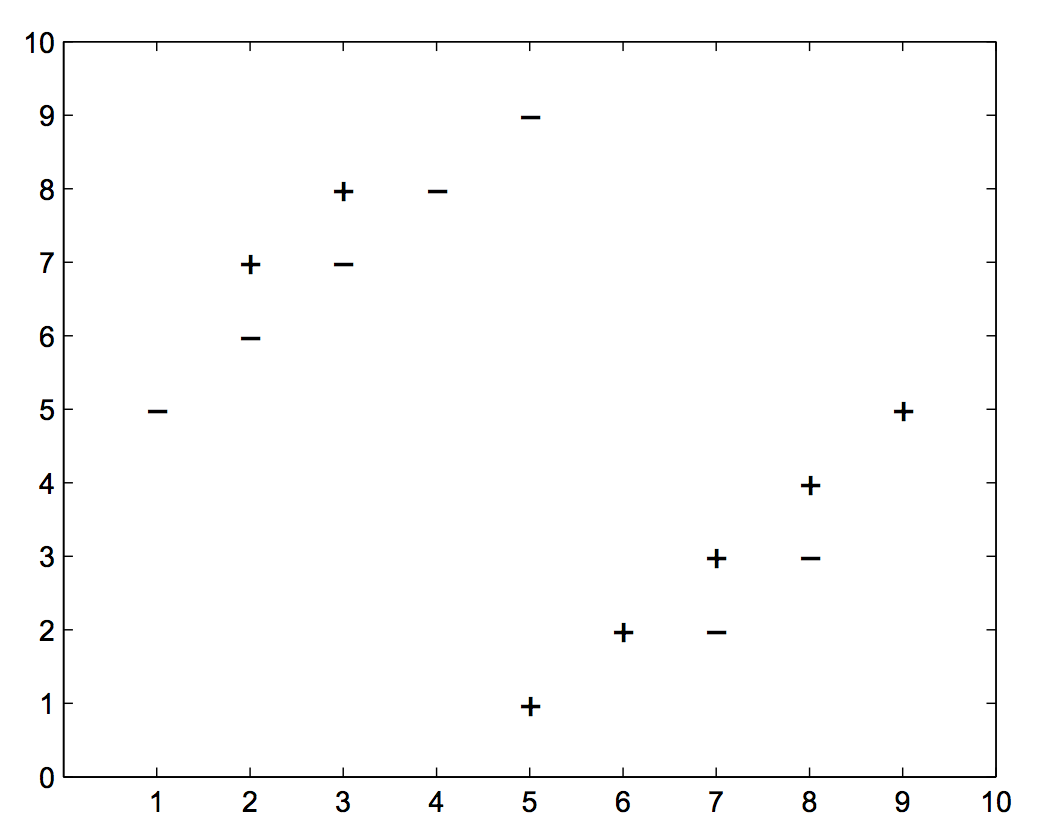
\includegraphics[width = 0.6\textwidth]{Q2_knn.png}
        \label{Q2_knn}
    \end{figure}

    \item \textbf{[3pt]} Consider a $k$-nearest neighbors binary classifier which assigns the class of a test point to be the class of the majority of the $k$-nearest neighbors, according to a Euclidean distance metric. Using the data set shown above to train the classifier and choosing $k=5$, which is the classification error on the training set? Assume that a point can be its own neighbor.
    
    Answer as a decimal with precision 4, e.g. (6.051, 0.1230, 1.234e+7)
    
    \begin{tcolorbox}[fit,height=1cm, width=4cm, blank, borderline={1pt}{-2pt},nobeforeafter]
    %solution
    \begin{center}\huge0.2857\end{center}
    \end{tcolorbox}
 
    
    
    \item \textbf{[3pt]} In the data set shown above, what is the value of $k$ that minimizes the training error? Note that a point can be its own neighbor. Let’s assume we use random-picking as the tie-breaking algorithm.
    
    \begin{tcolorbox}[fit,height=1cm, width=4cm, blank, borderline={1pt}{-2pt},nobeforeafter]
    %solution
    \begin{center}\huge1\end{center}
    \end{tcolorbox}

    
    
    \item \textbf{[3pt]} Assume we have a training set and a test set drawn from the same distribution, and we would like to classify points in the test set using a $k$-NN classifier. 
    
    \begin{enumerate}
        \item In order to minimize the classification error on this test set, we should always choose the value of $k$ which minimizes the training set error. 
    
    \textbf{Select one:}
    \begin{list}{}
        \item $\circle$ True
        \item $\blackcircle$ False
    \end{list}
    
    \item Instead of choosing the hyper-parameters by merely minimizing the training set error, some people would like to split the training-all data set into training and validation data set, and choose the hyper-parameters that lead to lower validation error. How do you think of this method? Justify your opinion with no more than 3 sentences.

    \textbf{Select one:}
    \begin{list}{}
        \item $\circle$ Good
        \item $\blackcircle$ No good
    \end{list}

    \textbf{NOTE: Please do not change the size of the following text box, and keep your answer in it. Thank you!} \\ \\
    \begin{tcolorbox}[fit,height=4cm, width=15cm, blank, borderline={1pt}{-2pt},nobeforeafter]
    \large
    Relying on just one validation set for tuning our hyperparameters resembles doing so by minimizing the training error, which isn't good since it doesn't work well on held out data. On the contrary, cross-validation would be a good approach, since we're constantly splitting our data into different sets, each time adjusting the hyperparameters. It is more likely that our method will generalize on unseen data.

    \end{tcolorbox} \\

    \end{enumerate}
    
    
    \item \textbf{[3pt]} Consider a binary $k$-NN classifier where $k=4$ and the two labels are ``triangle" and ``square".
    
    Consider classifying a new point $\xv =(1,1)$, where two of the $\xv$'s nearest neighbors are labeled ``triangle" and two are labeled ``square" as shown below.
    
    \begin{figure}[H]
        \centering
        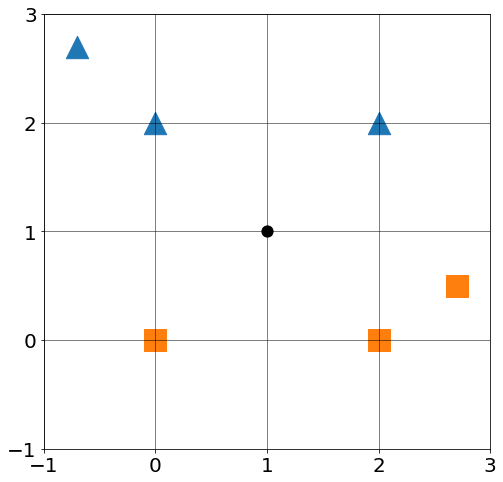
\includegraphics[width = 0.5\textwidth]{1-1-5.png}
        \label{Q_5knn}
    \end{figure}
    
    Which of the following methods can be used to break ties or avoid ties on this dataset?
    
    \begin{enumerate}
        \item Assign x the label of its nearest neighbor
        \item Flip a coin to randomly assign a label to $\xv$ (from the labels of its 4 closest points)
        \item Use $k = 3$ instead
        \item Use $k = 5$ instead
    \end{enumerate}

    \textbf{Select one:}
    \begin{list}{}
        \item $\circle$ a only
        \item $\circle$ b only
        \item $\circle$ b,c,d
        \item $\blackcircle$ b,d
        \item $\circle$ d only
        \item $\circle$ a,b,c,d
        \item $\circle$ None of the above
    \end{list}
    
 
    
    \newpage
    \item \textbf{[2pt]} Consider the following data concerning the relationship between academic performance and salary after graduation. High school GPA and university GPA are two numerical variables (predictors) and salary is the numerical target. Note that salary is measured in thousands of dollars per year.
    
    \begin{table}[H]
        \centering
        \begin{tabular}{cccc}
            \textbf{Student ID} & \textbf{High School GPA} & \textbf{University GPA} & \textbf{Salary} \\
            1 & 2.2 & 3.4 & 45 \\
            2 & 3.9 & 2.9 & 55 \\
            3 & 3.7 & 3.6 & 91 \\
            4 & 4.0 & 4.0 & 142 \\
            5 & 2.8 & 3.5 & 88 \\
            6 & 3.5 & 1.0 & 2600 \\
            7 & 3.8 & 4.0 & 163 \\
            8 & 3.1 & 2.5 & 67 \\
            9 & 3.5 & 3.6 & unknown \\
        \end{tabular}
        \label{tab:my_label}
    \end{table}
    
    Among Students 1 to 8, who is the nearest neighbor to Student 9, using Euclidean distance?
    
    Answer the Student ID only.

    \begin{tcolorbox}[fit,height=1cm, width=4cm, blank, borderline={1pt}{-2pt},nobeforeafter]
    %solution
    \begin{center}\huge3\end{center}
    \end{tcolorbox}

 
    
    
    \item \textbf{[3pt]} In the data set shown above, our task is to predict the salary Student 9 earns after graduation. We apply $k$-NN to this regression problem: the prediction for the numerical target (salary in this example) is equal to the average of salaries for the top $k$ nearest neighbors. 
    
    If $k=3$, what is our prediction for Student 9's salary?
    
    Round your answer to the nearest integer. Be sure to use the same unit of measure (thousands of dollars per year) as the table above.
    
    \begin{tcolorbox}[fit,height=1cm, width=4cm, blank, borderline={1pt}{-2pt},nobeforeafter]
    %solution
    \begin{center}\huge132\end{center}
    \end{tcolorbox}
    
    

\newpage
    \item \textbf{[3pt]} Suppose that the first 8 students shown above are only a subset of your full training data set, which consists of 10,000 students. We apply KNN regression using Euclidean distance to this problem and we define training loss on this full data set to be the mean squared error (MSE) of salary.

    Now consider the possible consequences of modifying the data in various ways. Which of the following changes \textbf{could} have an effect on training loss on the full data set as measured by mean squared error (MSE) of salary? Select all that apply.
    
    
        
    \textbf{Select all that apply:}
    \begin{list}{}
        \item $\blacksquare$ Rescaling only ``High School GPA" to be a percentage of 4.0
        \item $\blacksquare$ Rescaling only ``University GPA" to be a percentage of 4.0
        \item $\square$ Rescaling both ``High School GPA" and ``University GPA", so that each is a percentage of 4.0 (scale by the same percentage).
        \item $\square$ None of the above.
    \end{list}

    
    
    \item \textbf{[3pt]} In this question, we would like to compare the differences among KNN, the perceptron algorithm, and linear regression. Please select all that apply.
    
    \textbf{Select all that apply:}
    \begin{list}{}
        \item $\blacksquare$ For classification tasks, both KNN and the perceptron algorithm can have linear decision boundaries.
        \item $\square$ For classification tasks, both KNN and the perceptron algorithm always have linear decision boundaries.
        \item $\blacksquare$ All three models can be susceptible to overfitting.
        \item $\square$ In all three models, after the training is completed, we must store the training data to make predictions on the test data.
        \item $\square$ None of the above.
    \end{list}

    

    \item \textbf{[3pt]} Please select all that apply about kNN in the following options.

    \textbf{Select all that apply:}
    \begin{list}{}
        \item $\blacksquare$ Large $k$ gives a smoother decision boundary
        \item $\blacksquare$ To reduce the impact of noise or outliers in our data, we should increase the value $k$.
        \item $\square$ If we make $k$ too large, we could end up overfitting the data.
        \item $\blacksquare$ We can use cross-validation to help us select the value of $k$.
        \item $\square$ We should never select the $k$ that minimizes the error on the validation dataset.
        \item $\square$ None of the above.
    \end{list}

    
    
    \clearpage
\end{enumerate}
